\documentclass[11pt,english]{article}
\usepackage[T1]{fontenc}
\usepackage{babel}
\usepackage{graphicx}
\graphicspath{{images/}}
\usepackage{url}
\usepackage{hyperref}
\hypersetup{linktocpage}
\usepackage{booktabs}
\usepackage[vlined,algoruled]{algorithm2e}
\usepackage{amsthm}
\theoremstyle{definition}
\usepackage{booktabs}
\newtheorem{definition}{Definition}[section]
\author{Overclock Labs}
\title{Akash Network: Decentralized Cloud Infrastructure Marketplace}
\date{\today}
\begin{document}
\maketitle
\begin{center} Version 0.0.4 \end{center}
\begin{center} 
\small{
\textit{Note: The Akash Network is an active research project and new versions of this paper will manifest at \href{https://akash.network}{akash.network}. For comments and suggestions please reach out at \href{mailto:research@akash.network}{research@akash.network}}}
\end{center}

\abstract{
Cloud computing --- the process of offloading work to remote servers --- is inherently broken. While it mostly works as advertised, we've found that inefficiencies still plague the system. The products produced by the major cloud providers are usable but they are limited to shortcomings that can be solved today with advancements in container technology and a powerful token economy. The purpose of this white paper is to put forward our plan for a cloud services market called Akash Network, the worlds first global spot market for cloud computing.

We see a future where the global cloud infrastructure of the world is decentralized and distributed between all cloud service providers; a market that deploys and liquidates (increasingly commoditized) data center compute in a secure, fast and transparently spot priced manner. Services are sold in a democratic but unified ecosystem that anyone can use. 

In this paper, we present Akash, cloud infrastructure network that is decentralized, competitive, and able to distribute applications between multiple cloud service providers around the globe. The paper will introduce the state of the existing market, outline how we are using latest developments in serverless container orchestration to combat these issues, the basics of and the necessity of the networks native token, AKASH, and finally our roadmap for launch. 
}
\clearpage
\setcounter{tocdepth}{2}
\tableofcontents
\clearpage
\listoffigures
\clearpage

\section{Introduction}

The Akash Network (\textit{Akash}) is a secure, transparent, and decentralized cloud computing marketplace that connects those who need computing resources (\textit{clients}) with those that have computing capacity to lease (\textit{providers}).

Akash acts as a "super" cloud platform (\textit{supercloud}) - providing a unified layer above all providers on the marketplace so as to present clients with a single cloud platform, regardless of which particular provider they may be using. 

Clients use Akash because of its cost advantage, usability, and flexibility to move between cloud providers, and the performance benefits of global deployments.  Providers use Akash because it allows them to earn profits from either dedicated or temporarily-unused capacity.

\subsection{A Troubled Industry}

By 2020, cloud infrastructure providers will account for \textbf{53\%} of global internet traffic\cite{CISCO}, out of which Amazon, Google, and Microsoft will deliver \textbf{80\% }of the payload\cite{FORRESTER}.

While the cloud will deliver the majority of the workloads, the future of the internet stands at a risk of being consolidated, centralized, and at the mercy of these three providers.

The primary driver for cloud adoption is the promise of flexibility and cost advantage, but the reality is that the products offered by cloud providers are overpriced, complicated, and lock clients into ecosystems that limit their ability to innovate, compete, and have sovereignty over their infrastructure needs.

The difference in capital expenditure of purchasing hardware and leasing datacenters between running in the cloud and self managing (on-premise) is marginal; however, the cloud providers have a significant advantage with operating expenditure because of their investments in automation with minimal human touch.

Even though running computing on-premise can offer much better flexibility, performance, and security, organizations are abandoning their datacenter operations and migrating to the cloud because they are finding it increasingly hard to justify the operating costs due to lack of adequate automation along with low utilization footprint. Idle, underutilized servers prove to be costly and wasteful. Analysts estimate that as many as 85\% of servers in practice have underutilized capacity \cite{NYT} \cite{MCKINSEY} \cite{ACCENTURE} \cite{ANTHESIS}.


Cloud providers drive margins by building hyper-scale installations, i.e, consolidating resources in few datacenters for economic efficiency, and cross-selling fully managed backend services, such as databases, cache stores, API gateways, etc.

Being hyper-scale allows them to oversubscribe their customers, hence driving higher margins but creates single-points for failures. Geographically distributed workloads offer much reliability and end-user performance; however, the cloud providers make it extremely hard for clients to be multi-regional because it doesn't work in their best interest.

The cloud providers prefer customers to deploy their applications in a single datacenter and penalize them for being cross-regional or multi-zonal, usually through hefty bandwidth fees and variable regional pricing. This is why AWS' pricing model is different for each region for the same exact resource.

Even though selling instances is lucrative, Cloud Providers usually charge a small amount for instances compared to the premium they charge for managed backend services (\textit{PaaS}); analogous to the old burgers-and-fries model where a restaurant needs to sell burgers at a loss so that they can sell the more addictive fries at a high margin. 

The PaaS services sold by the providers tend to be white-labeled open source projects where the original authors are never incentivized, and the cloud providers have no incentive to evolve the product. For example, AWS' ElastiCache is a white-labeled open source software called Redis. Redis is an open source project --- much loved by developers --- written by Salvatore Sanfilippo and maintained by Redis Labs.

As of the writing of this paper, a managed Redis server, in US East (Ohio) running on \textit{r3.8xlarge} is priced at \$31,449/yr \cite{AECPRICING} whereas the same instance without Redis costs \$18,385/yr \cite{EC2PRICING}. The extra \$13,064 just for a "piece of mind" to the customer. Neither Sanfilippo or Redis Labs are incentivized for the efforts. 

Also, more services mean more dependent the customer is on the cloud provider. The complexity introduced by increasing amounts of features, service availability, and codification using non-standard APIs lead to customers being locked in by the cloud vendors, preventing clients from exploring other better options in the marketplace while inhibiting innovation.

This model adopted by the providers stifles innovation as it dramatically reduces the chance of an open source project from succeeding. Cloud providers effectively act as middle-men that set the rules of engagement for the industry while making a no contribution to society on the whole.


\section{The Akash Network}
The foundational design objective of the Akash Network is to maintain a low barrier to entry for providers while at the same time ensuring that clients can trust the resources that the platform offers them.  To achieve this, the system requires a publicly-verifiable record of transactions within the network. To that end, the Akash Network is implemented using blockchain technologies as a means of achieving consensus on the veracity of a distributed database.

Akash is, first and foremost, a platform that allows clients to procure resources from providers.  This is enabled by a blockchain-powered distributed exchange where clients post their desired resources for providers to bid on. The currency of this marketplace is a digital token, the Akash (AKASH), whose ledger is stored on a blockchain.

Akash is a cloud platform for real-world applications. The requirements of such applications include:

\begin{itemize}
  \item Many workloads deployed across any number of datacenters.
  \item Connectivity restrictions which prevent unwanted access to workloads.
  \item Self-managed so that operators do not need to constantly tend to deployments.
\end{itemize}

To support running workloads on procured resources, Akash includes a peer-to-peer protocol for distributing workloads and deployment configuration to and between a client's providers.

Workloads in Akash are defined as Docker containers. Docker containers allow for highly-isolated and configurable execution environments, and are already part of many cloud-based deployments today.
\begin{figure}[hbt]
\centering
  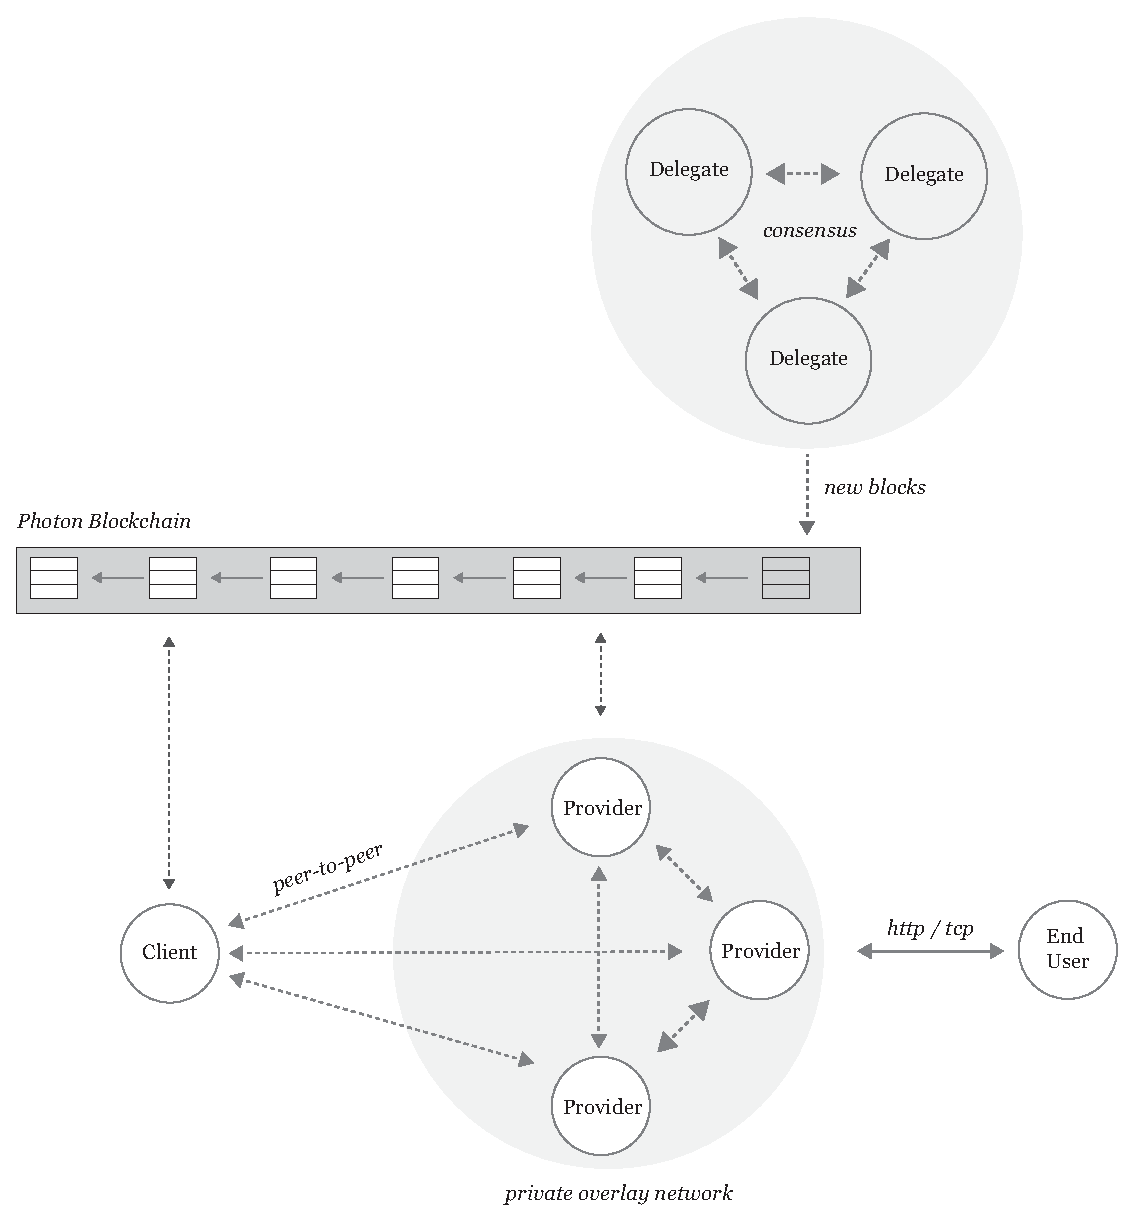
\includegraphics[width=0.8\textwidth]{overview}
  \caption{Illustration of on-chain and off-chain interactions amongst various participants in the Akash network}
\end{figure}

\subsection{The Akash Blockchain}
The Akash blockchain provides a layer of trust in a decentralized and trustless environment. Clients inherently trust today's large infrastructure Providers based primarily on the brand equity they've built over years.Akash does not and should not require that same leap of faith, since any Provider with capacity can compete to offer services on Akash. Instead, the blockchain earns trust via an open and transparent platform. Data on the chain is an immutable and public record of all transactions, including each Provider's fulfillment history. 

Akash is also politically decentralized.  No single entity controls the network and no intermediary facilitates transactions. Therefore no entity is incentivized to control or to extract marginal revenue from the network.  As an example, a large company such as Coca-Cola can participate in the network as a Provider, providing compute to another large company or to an individual developer, yet all three parties are on equal footing in the network.


\subsection{The Akash Token, AKASH}

The Akash Token (AKASH) is used to simplify the exchange of value and align economic incentives with proper user behavior. The Akash token is the marketplace currency used to pay for leased compute infrastructure on Akash's decentralized network. Our token serves two primary functions in Akash's ecosystem.

In a market that is expected to be \textbf{\$737 billion}, with well over 21\% annual growth \cite{GARTNER}, the liquidity of AKASH will be matched by the demand for compute power. Along this line of thought, we have full confidence in the network and for AKASH to achieve maximum liquidity for its early adopters and end state user. 

\subsubsection{Staking}
The stability of the Akash network relies on a staking system that prevents bad actors from abusing our system. A staking system provides a prohibitive monetary disincentive for bad actors who consider participating in our network. The risk of fraudulent behavior is highest when new, unknown providers join our network. Rather than requiring a centralized or federated approval process for new accounts, the Akash network allows anyone to join.

When a new provider chooses to offer its resources on the Akash network, rather than being approved, it must stake a meaningful value on the network in Akash tokens. There is no minimum stake amount, but participation in Akash Network governance is proportional to a provider's stake, taken as a fraction of the sum of all stakes. Additionally, stake contribution is factored into a provider's reputation score, which tenants may use as a deployment criterion.

\subsubsection{Global Payments}

Akash tokens mitigate the foreign exchange risk that usually results from cross-border payments. Taking the place of fiat for these transactions, Akash tokens simplify the exchange of value in the cloud infrastructure industry. Our matching engine competitively prices each container compute against a prevailing market amount of Akash tokens. When a tenant is matched with a provider, the tenant pays Akash tokens to the network, which are subsequently paid to the provider according to the terms of the lease.

\subsection{Protocol}
\begin{enumerate}
  \item Tenants define desired infrastructure, workloads to run on infrastructure, and how workloads can connect to one another. Desired lifetime of resources is expressed via collateral requirements.
  \item Orders are generated from the tenant's definition.
  \item Datacenters bid on open orders.
  \item The bid with lowest price gets matched with order to create a lease.
  \item Once lease is reached, workloads and topology are delivered to datacenter.
  \item Datacenter deploy workloads and allow connectivity as specified by the tenant.
  \item If a datacenter fails to maintain lease, collateral is transferred to tenant, and a new order is crated for the desired resources.
  \item A tenant can close any active deployment at any time
\end{enumerate}

\section{Marketplace}

\begin{figure}[hbt]
  \centering
  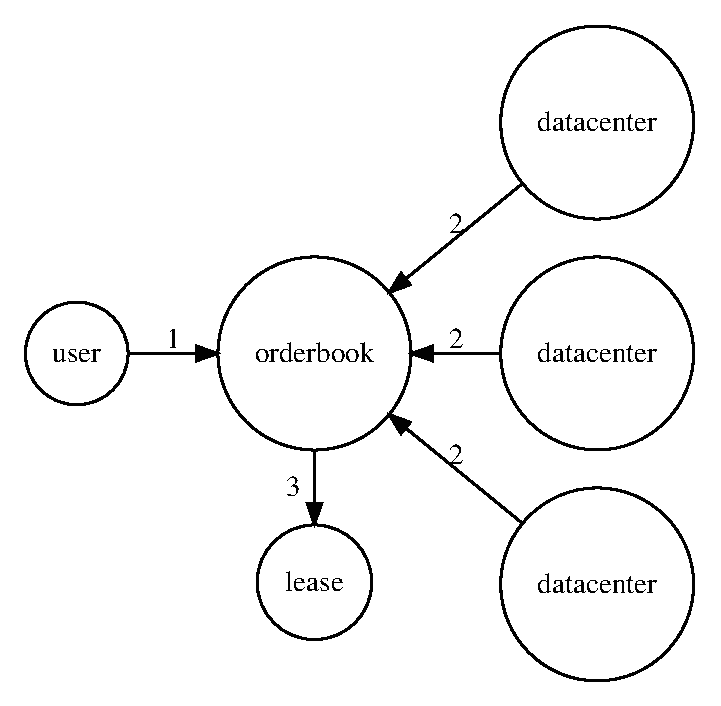
\includegraphics[width=0.5\textwidth]{marketplace}
  \caption{Summary of procurement from Marketplace. (1) User's deployment order is posted to the orderbook (2)
Datacenters posts eligible fulfillment orders for the deployment order (3) The best fulfillment order is matched with the deployment order, creating a new lease.
}
\end{figure}

Infrastructure procurement --- the process through which clients lease infrastructure from providers --- on Akash is implemented through a decentralized exchange (\textit{marketplace}).

The marketplace consists of a public order book and a matching algorithm. Clients place \textit{deployment} orders, which contain a specification of the client's service needs, and datacenters place \textit{fulfillment} orders to bid on deployment orders. Deployment orders include the maximum amount the client is willing to pay for a fixed number of computing units (as measured by memory, cpu, storage, and bandwidth) for a specific amount of time; fulfillment orders declare the price that the provider will provide the resources for.

Deployment orders are \textit{open} for a client-defined length of time, as measured to the second. While the deployment order is open, providers may post fulfillment orders to bid on it.

A fulfilment order is eligible to match with a deployment order if the fulfillment order satisfies all minimum specifications of the deployment order. Given a deployment order and a set of eligible fulfilment orders, the fulfilment order offering the lowest price will be matched with the deployment order. If multiple fulfilment orders are eligible for a match and offer the same price, the fulfilment order placed first will be matched with the deployment order.

Businesses and individual consumers will want and need to protect how they are publicly displaying their use of compute power. To guard against competitor data mining and other attack vectors, a homomorphic encryption layer is added. 

A \textit{lease} is created when a match occurs between a deployment and fulfillment order. The lease contains references to the deployment and fulfilment orders. Leases will be the binding agent in fulfilling a deployment. 

\subsection{Actors}

\begin{description}
\item [Tenant] \textit{tenant} hosting an application on the Akash network.
\item [Datacenter] Each \textit{datacenter} will host an agent which is a mediator between the with the Akash Network and datecenter-local infrastructure. The datacenter agent is responsible for:
\begin{itemize}
  \item Bidding on orders fulfillable by the datacenter.
  \item Managing managing active leases it is a provider for.
\end{itemize}
\item [Validator] An Akash node that is elected to be a \textit{validator} in the \textit{DPoS} consensus scheme.
\item [Marketplace Facilitator] Marketplace \textit{facilitators} maintain the distributed exchange (marketplace). Validators will initially perform this function.
\end{description}

\subsection{Data Structures}


\begin{description}
	\item [ComputeUnit] \textit{ComputeUnit} defines the workload parameters.
	\begin{itemize}
	\item cpu, number of vCPUs
	\item memory, amount of memory in GB
	\item disk, amount of block storage in GB
	\end{itemize}
	\item [ResourceGroup] \textit{ResourceGroup} represents a group of \textit{ComputeUnit}s.
	\begin{itemize}
		\item compute, \textit{ComputeUnit} definition.
		\item price, price of \textit{ComputeUnit} per time unit.
		\item collateral	, collateral per \textit{ComputeUnit}.
		\item count, number of defined \textit{ComputeUnit}s.
	\end{itemize}
	\item [Deployment] A \textit{Deployment} represents the state of a \textit{tenant}'s application. It includes desired infrastructure and pricing parameters, as well as workload definitions and connectivity.
	\begin{itemize}
	\item infrastructure, list of deployment infrastructure definitions.
	\item wait-duration, amount of time to wait before matching generated orders with fulfillments.
	\end{itemize}
	\item [DeploymentInfrastructure] \textit{DeploymentInfrastructure} represents a set of resources (including pricing) that a \textit{tenant} would like to be provisioned in a single \textit{datacenter}. \textit{Orders} are created from \textit{deployment infrastructure} as necessary.
	\begin{itemize}
	\item region, geographic region of \textit{datacenter}.
	\item persist, whether or not to maintain active lease if current lease is broken.
	\item resources, list of resource groups for this \textit{datacenter}.
	\end{itemize}
	Within the resources list, resource group fields are interpreted as follows:
	\begin{itemize}
		\item price, maximum price \textit{tenant} is willing to pay.
		\item collateral, amount of collateral that the \textit{datacenter} must post when creating a \textit{fulfillment}.
	\end{itemize}
	\item [Order] A Order is generated for each \textit{DeploymentInfrastructure} present in the \textit{deployment}.
	\begin{itemize}
		\item region, geographic region of \textit{datacenter}.
		\item resources,	 list of \textit{ResourceGroup}s for this \textit{datacenter}.
		\item wait-duration, number of blocks to wait before matching the order with \textit{fulfillments}.
	\end{itemize}
	\item [Fulfillment] A \textit{Fulfillment} represents a datacenter's interest in providing the resources requested in a order.
	\begin{itemize}
		\item order, ID of \textit{order} which is being bid on.
		\item resources, list of \textit{ResourceGroup}s for this \textit{datacenter}.
	\end{itemize}
	The resources list must match the order's resources list for each resource group with the following rules:
	\begin{itemize}
		\item the \textit{compute}, \textit{count}, \textit{collateral} fields must be the same.
		\item the price field represents the \textit{datacenter}'s offering price and must be less than or equal to the \textit{order}'s price.
		The total collateral required to post a \textit{fulfillment} is the sum of collateral fields present in the \textit{order}'s resources list.
	\end{itemize}
	\item [Lease] A \textit{Lease} represents a matching order and fulfillment.
	\begin{itemize}
		\item deployment-order, ID of \textit{order}.
		\item fulfillment-order,	 ID of \textit{fulfillment}.
	\end{itemize}
	\item [LeaseConfirmation] A \textit{LeaseConfirmation} represents a confirmation that the resources are being provided by the datacenter. Its creation may initiate a transfer of tokens from the \textit{tenant} to the \textit{datacenter}.
	\begin{itemize}
		\item lease, ID of \textit{lease} being confirmed.
	\end{itemize}
\end{description}

\subsection{Transactions}
\begin{description}
	\item [SubmitDeployment] Sent by a \textit{tenant} to deploy their application on Akash. A \textit{order} will be created for each datacenter configuration described in the \textit{deployment}.
	\item [UpdateDeployment] Sent by a \textit{tenant} to update their application on Akash.
	\item [CloseDeployment] Sent by a \textit{tenant} to close their application on Akash.
	\item [DeploymentClosed] Sent by a \textit{facilitator} after the \textit{deployments}' \textit{datacenter}'s confirm the \textit{deployments}' resources have been reset.
	\item [SubmitFulfillment] Sent by a \textit{datacenter} to bid on a order.
	\item [CancelFulfillment] Sent by a \textit{datacenter} to cancel an existing \textit{fulfillment}.
	\item [SubmitLeaseConfirmation] Sent by a \textit{datacenter} to confirm a \textit{lease} that it is engaged in. This should be called once every \textit{reconfirmation period} rounds.
	\item [SubmitLease] Sent by a \textit{validator} to match a order with a \textit{fulfillment}.
	\item [SubmitStaleLease] Sent by a \textit{validator} after finding a lease that has not been confirmed in \textit{reconfirmation period} rounds.
	\item 
\end{description}

\section{Deployment}
Once resources have been procured, clients must distribute their workloads to providers so that they can execute on the leased resources.  We refer to the current state of the client's workloads on the Akash Network as a \textit{deployment}.

A user describes their desired deployment in a \textit{manifest}.  The manifest is written in a declarative file format that contains workload definitions, configuration, and connection rules.  Providers use workload definitions and configuration to execute the workloads on the resources they are providing, and use the connection rules to build an overlay network and firewall configurations.

A hash of the manifest is known as the deployment \textit{version} and is stored on the blockchain-based distributed database.
\subsection{Manifest Distribution}
	The manifest contains sensitive information which should only be shared with participants of the deployment.  This poses a problem for self-managed deployments - Akash must distribute the workload definition autonomously, without revealing its contents to unnecessary participants.

To address these issues, we devised a peer-to-peer file sharing scheme in which lease participants distribute the manifest to one another as needed.  The protocol runs off-chain over a TLS connection; each participant can verify the manifest they received by computing its hash and comparing this with the deployment version that is stored on the blockchain-backed distributed database.

In addition to providing private, secure, autonomous manifest distribution, the peer-to-peer protocol also enables fast distribution of large manifests to a large number of datacenters.
\subsection{Overlay Network}

\begin{figure}[h]
\centering
  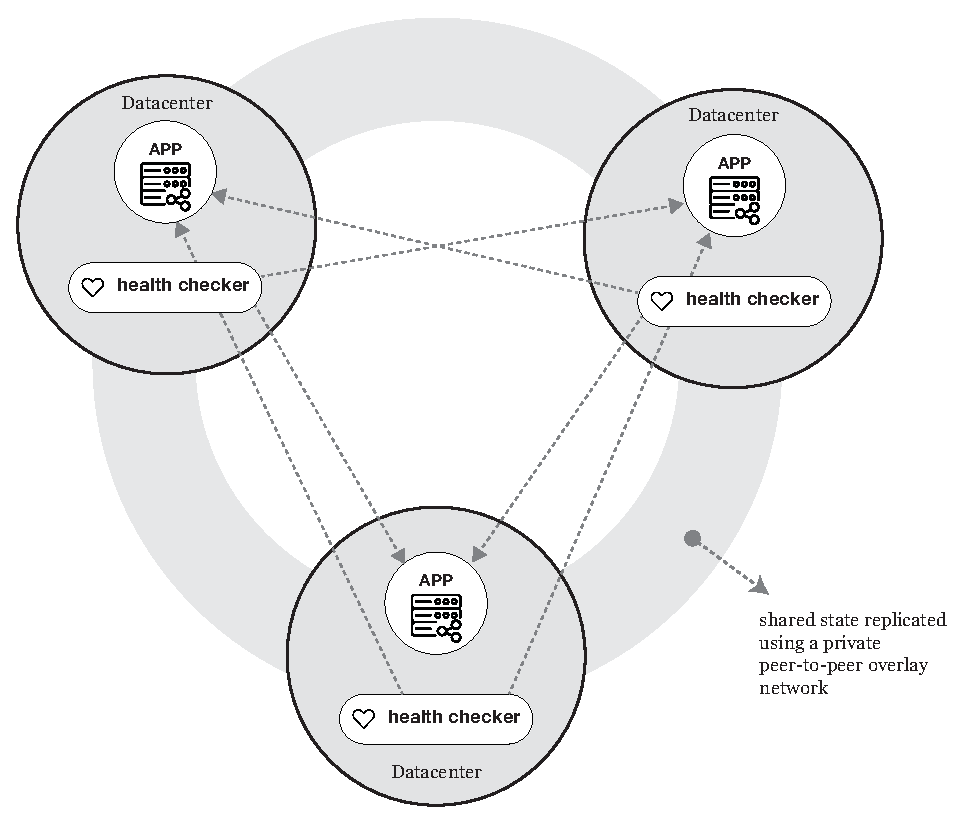
\includegraphics[width=0.6\linewidth]{overlay}
  \caption{Illustration of Akash's overlay network}
\end{figure}

By default, a workload's network is isolated - nothing can connect to it. While this is secure, it is not practical for real-world applications. For example, consider a simple web application: end-user browsers should have access to the web tier workload, and the web tier needs to communicate to the database workload. Furthermore, the web tier may not be hosted in the same datacenter as the database.

On the Akash Network, clients can selectively allow communications to and between workloads by defining a connection topology within the manifest. Datacenters use this topology to configure firewall rules and to create a secure network between individual workloads as needed.

To support secure cross-datacenter communications, providers expose workloads to each other through a mTLS tunnel. Each workload-to-workload connection uses a distinct tunnel.

Before establishing these tunnels, providers generate a TLS certificate for each required tunnel and exchange these certificates with the necessary peer providers.  Each provider's root certificate is stored on the blockchain-based distributed database, enabling peers to verify the authenticity of the certificates it receives.

Once certificates are exchanged, providers establish an authenticated tunnel and connect the workload's network to it.  All of this is transparent to the workloads themselves - they can connect to one another through stable addresses and standard protocols.

\section{Automation}
The dynamic nature of cloud infrastructure is both a blessing and a curse for operations management.  That new resources can be provisioned at will is a blessing; the exploding management overhead and complexity of said resources is a curse.  The goal of \textit{DevOps} --- the practice of managing deployments programmatically --- is to alleviate the pain points of cloud infrastructure by leveraging its strengths.

The Akash Network was built from the ground up to provide DevOps engineers with a simple but powerful toolset for creating highly-automated deployments.  The toolset is comprised of the primitives that enable non-management applications --- generic workloads and overlay networks --- and can be leveraged to create autonomous, self-managed systems.

Self-managed deployments on Akash are a simple matter of creating workloads that manage their own deployment themselves.  A DevOps engineer may employ a workload that updates DNS entries as providers join or leave the deployment; tests response times of web tier applications; and scales up and down infrastructure (in accordance with permissions and constraints defined by the client) as needed based on any number of input metrics.  The "management tier" may be spread across all datacenters for a deployment, with global state maintained by a distributed database running over the secure overlay network.
\subsection{Example: Latency-Optimized Deployment}
\begin{figure}[h]
\centering
  \includegraphics[width=0.8\linewidth]{latency-general}
  \caption{Illustration of slower performance due to higher latencies for end-users distributed across the globe for a single datacenter deployment}
\end{figure}
\begin{figure}[h]
\centering
  \includegraphics[width=0.8\linewidth]{latency-photon}
  \caption{Illustration of improved network performance by dynamically distributing workloads and their state across datacenters in close proximity to the end-users}
\end{figure}
Many web-based applications are \textit{latency-sensitive} - lower response times from application servers translates into a dramatically improved end-user experience. Modern deployments of such applications employ \textit{content delivery networks (CDNs)} to deliver static content such as images to end users quickly.

CDNs provide reduced latency by distributing content so that it is geographically close to the users that are accessing it.  Deployments on the Akash Network can not only replicate this approach, but beat it - Akash gives clients the ability to place dynamic content close to an application's users.

To implement a self-managed \textit{dynamic delivery network} on Akash, a DevOps engineer would include a management tier in their deployment which monitors the geographical location of clients.  This management tier would add and remove datacenters across the globe, provisioning more resources in regions where user activity is high, and less resources in regions where user participation is low.

\subsection{Example: Machine Learning Deployment}

Machine learning applications employ a large number of nodes to parallelize computations involving large datasets.  They do their work in "batches" - there is no "steady state" of capacity that is required.

A machine learning application on Akash may use a management tier to proactively procure resources within a single datacenter. As a machine learning task begins, the management tier can "scale up" the number of nodes for it; when a task completes, the resources provisioned for it can be relinquished.
\begin{figure}[htp]
\centering
  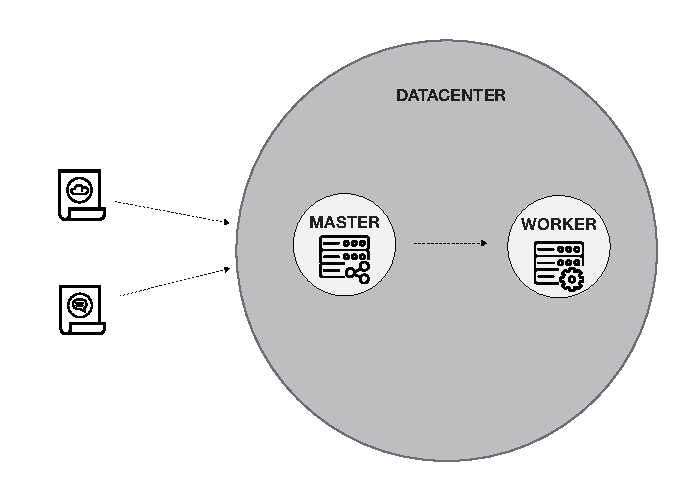
\includegraphics[width=0.4\textwidth]{batch-normal}
  \caption{A machine learning batch job under less load running a single master and single worker node}
\end{figure}
\begin{figure}[htp]
\centering
  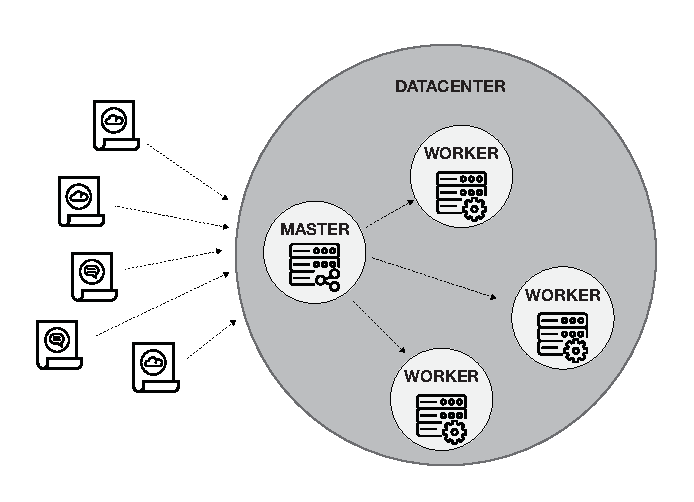
\includegraphics[width=0.4\textwidth]{batch-scale}
  \caption{A machine learning batch job under load running a single master and multiple worker nodes}
\end{figure}
\clearpage
\bibliography{biblio}
\bibliographystyle{plainnat}
\end{document}
